\section{Durchführung}
\label{sec:Durchführung}
In diesem Versuch werden, wie im \autoref{sec:Ziel} beschrieben, die Trägheitsmomente verschiedener Körper berechnet. 

\subsection{Vorbereitungsaufgaben}
\label{subsec:D_Va}
Zur Vorbereitung des Versuches sollten die Drehmomente $M_i$ einer Kraftwirkung von $F = \qty{0.1}{\newton}$ im Winkel von $\phi = \qty{45}{\degree}$
zu verschiedenen Abständen $r_i$ berechnet werden. Dazu wird die Formel $M = Fr\, \text{cos}(\frac{\pi}{2})$ genutzt. Die errechneten Werte können \autoref{tab:D_VA} entnommen werden.
\begin{table}[H]
    \centering
    \caption{Berechnete Werte der Vorbereitungsaufgabe.} 
    \label{tab:D_VA}
    \begin{tabular}{S[table-format = 2.1] S[table-format = 2.1]}
        \toprule
        $r_i \mathrm{/} \unit{\centi\metre}$ & $M_i \mathrm{/} \unit{{\milli\newton\metre}}$\\
        \midrule
        5    &  3.56 \\
        7.5  &  5.3  \\
        10   &  7.07 \\
        12.5 &  8.8  \\
        15   & 10.6  \\
        17.5 & 12.37 \\
        20   & 14.14 \\
        22.5 & 15.9  \\
        25   & 17.67 \\
        \bottomrule 
    \end{tabular}
\end{table}
\subsection{Experimentelle Bestimmung der Apparatkonstanten}
\label{subsec:D_const}
Zu Beginn werden die Winkelrichtgröße $D$ und das Eigenträgheitsmoment $I_D$ der Drill-Achse bestimmt. Dazu wird zunächst ein Stab an der Drill-Achse befestigt. Anschließend 
wird ein Newtonmeter senkrecht an dem Stab eingehängt. Die Drill-Achse wird nun mit dem Newtonmeter um $90\unit{\degree}$ asugelenkt. Die auf dem abzulesende Kraft wird notiert. Diese 
Messung wird mindestens zehn Mal durchgeführt und die Ergebnisse danach gemittelt. Dazu wird ebenfalls der Abstand der Aufhängung zur Drill-Achse notiert.
Aus diesen Werten kann die Winkelrichtgröße $D$ gemäß \autoref{eqn:Winkelrichtgröße} bestimmt werden.
Um das Eigenträgheitsmoment der Drill-Achse zu bestimmen, werden zwei Gewichte in symmetrischen Abständen an der Stange angebracht. Nun wird die Stange ausgelenkt, sodass sie schwingt.
Dabei wird die Schwingungsdauer für mehrere Perioden gemessen und gemittelt. Diese Messung wird für mindestens zehn verschiedene Abstände der Gewichte zur Drillachse wiederholt.
Aus dieser Messung kann das Eigenträgheitsmoment bestimmt werden.
\subsection{Experimentelle Bestimmung der Trägheitsmomente einfacher Körper}
\label{subsec:D_Körper}
Im ersten Teil der eigentlichen Messung soll das Trägheitsmoment zweier einfacher Körper bestimmt werden. Dazu werden diese Körper zunächst gewogen und abgemessen. Anschließend
werden die Körper auf der Drill-Achse angebracht. Wie zuvor, werden
die Körper um $90\unit{\degree}$ auf der Drill-Achse ausgelenkt. Es wird die Schwingungsdauer gemessen. Pro Körper werden zehn Messungen durchgeführt. Die Ergebnisse werden gemittelt.
\subsection{Experimentelle Bestimmung des Trägheitsmoments einer Modellpuppe}
\label{subsec:D_Figur}
Zuletzt werden die Trägheitsmomente einer Modellpuppe aus Holz in verschiedenen Stellungen bestimmt. Diese sind in \autoref{fig:D_subfig} zu sehen.
Die Holzpuppe wird an ihrem Stab in die Drill-Achse eingespannt. Zunächst wird sie in Stellung 1 gebracht, welche in \autoref{fig:D_Holzpuppe1} zusehen ist. In dieser Stellung wird die Figur fünf 
mal um $90\unit{\degree}$ und weitere fünf mal um $120\unit{\degree}$ ausgelenkt. Dabei werden je drei Periodendauern gemessen und der Mittelwert gebildet. Dieses Verfahren wird für 
Stellung 2, welche \autoref{fig:D_Holzpuppe2} entnommen werden kenn, erneut durchgeführt. 

\begin{figure}
    \centering
    \begin{subfigure}{0.4\textwidth}
        \centering
        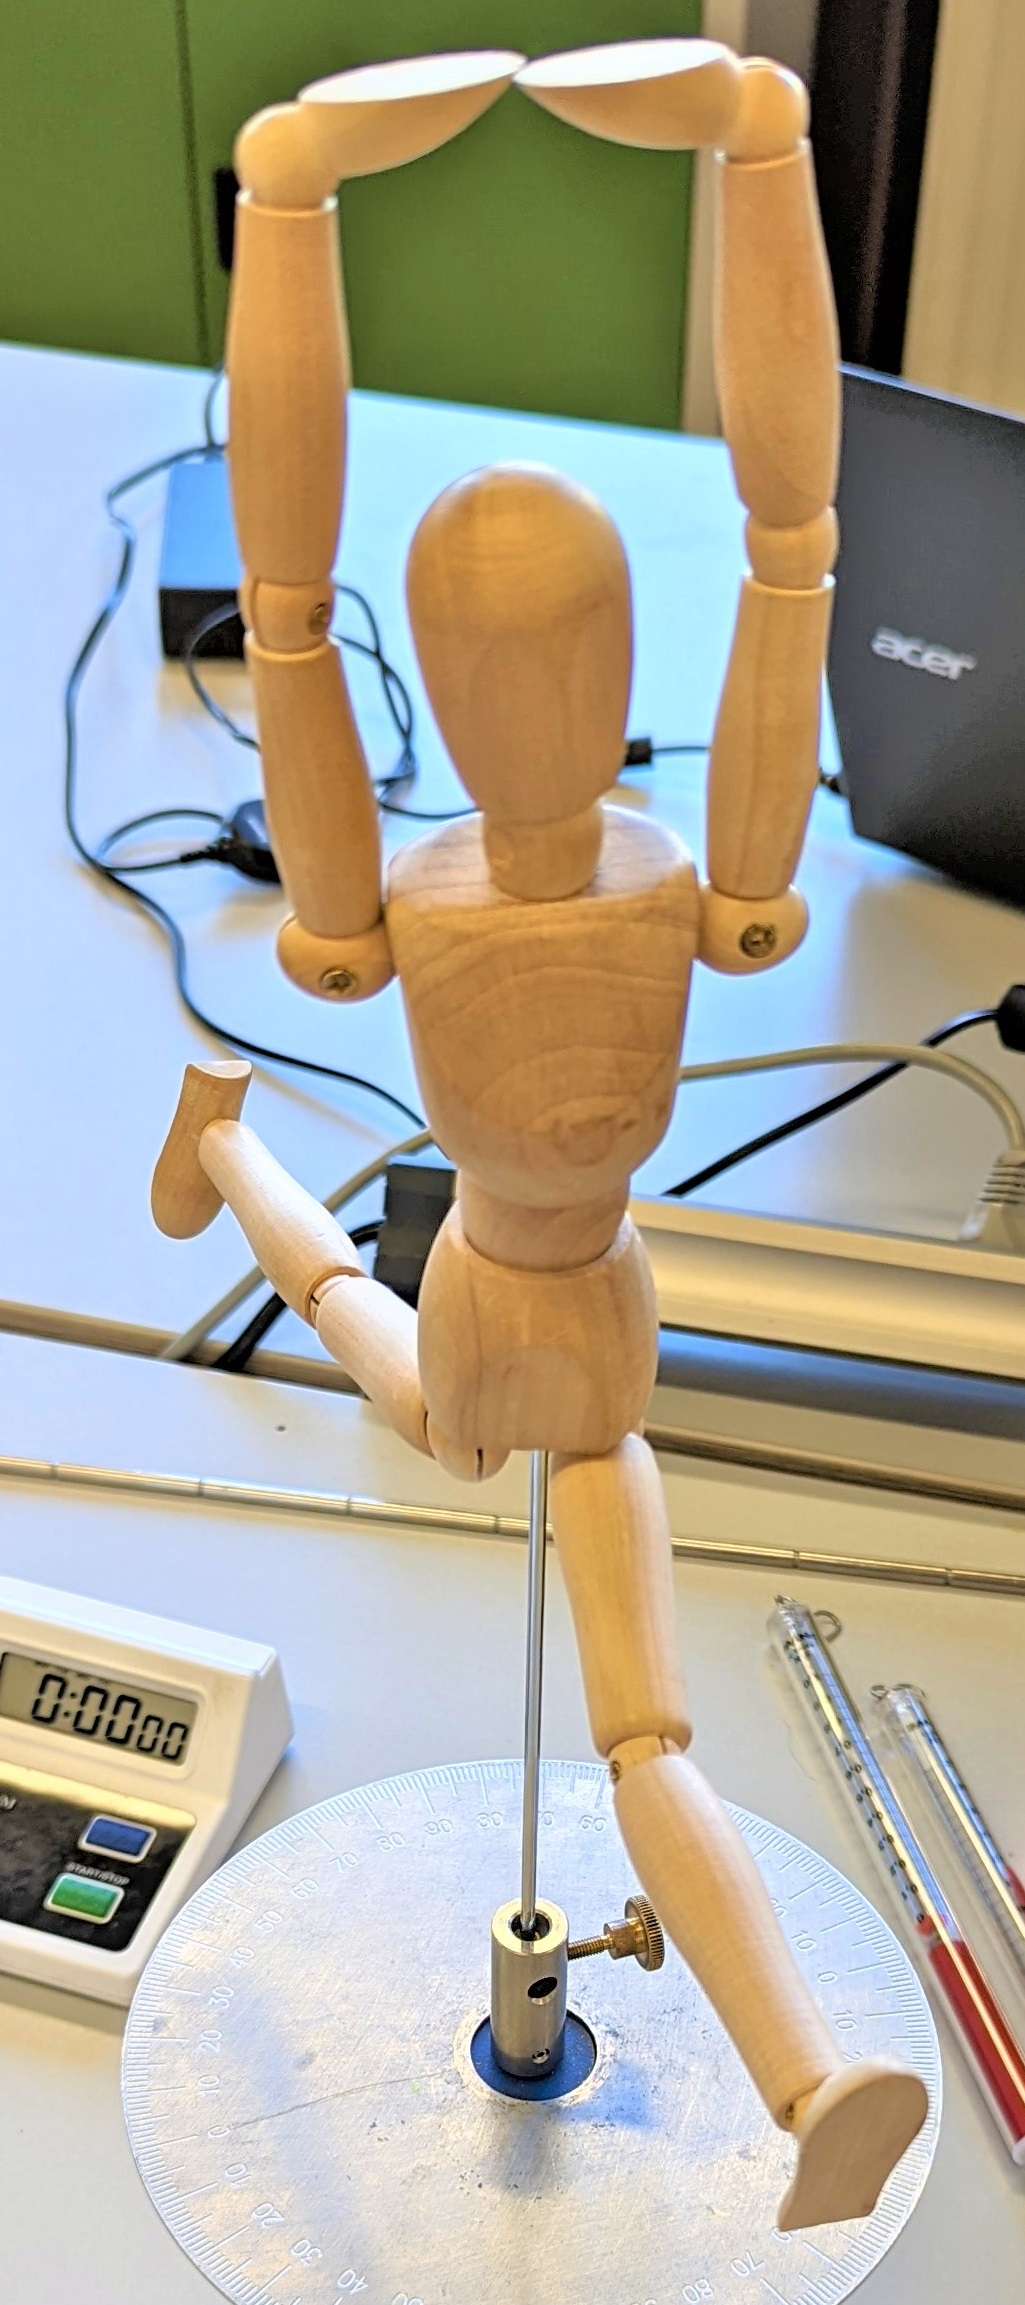
\includegraphics[width=0.65\textwidth]{content/Ballet3.jpg}
        \caption{Stellung 1}
        \label{fig:D_Holzpuppe1}
    \end{subfigure}
    \hfill
    \begin{subfigure}{0.48\textwidth}
        \centering
        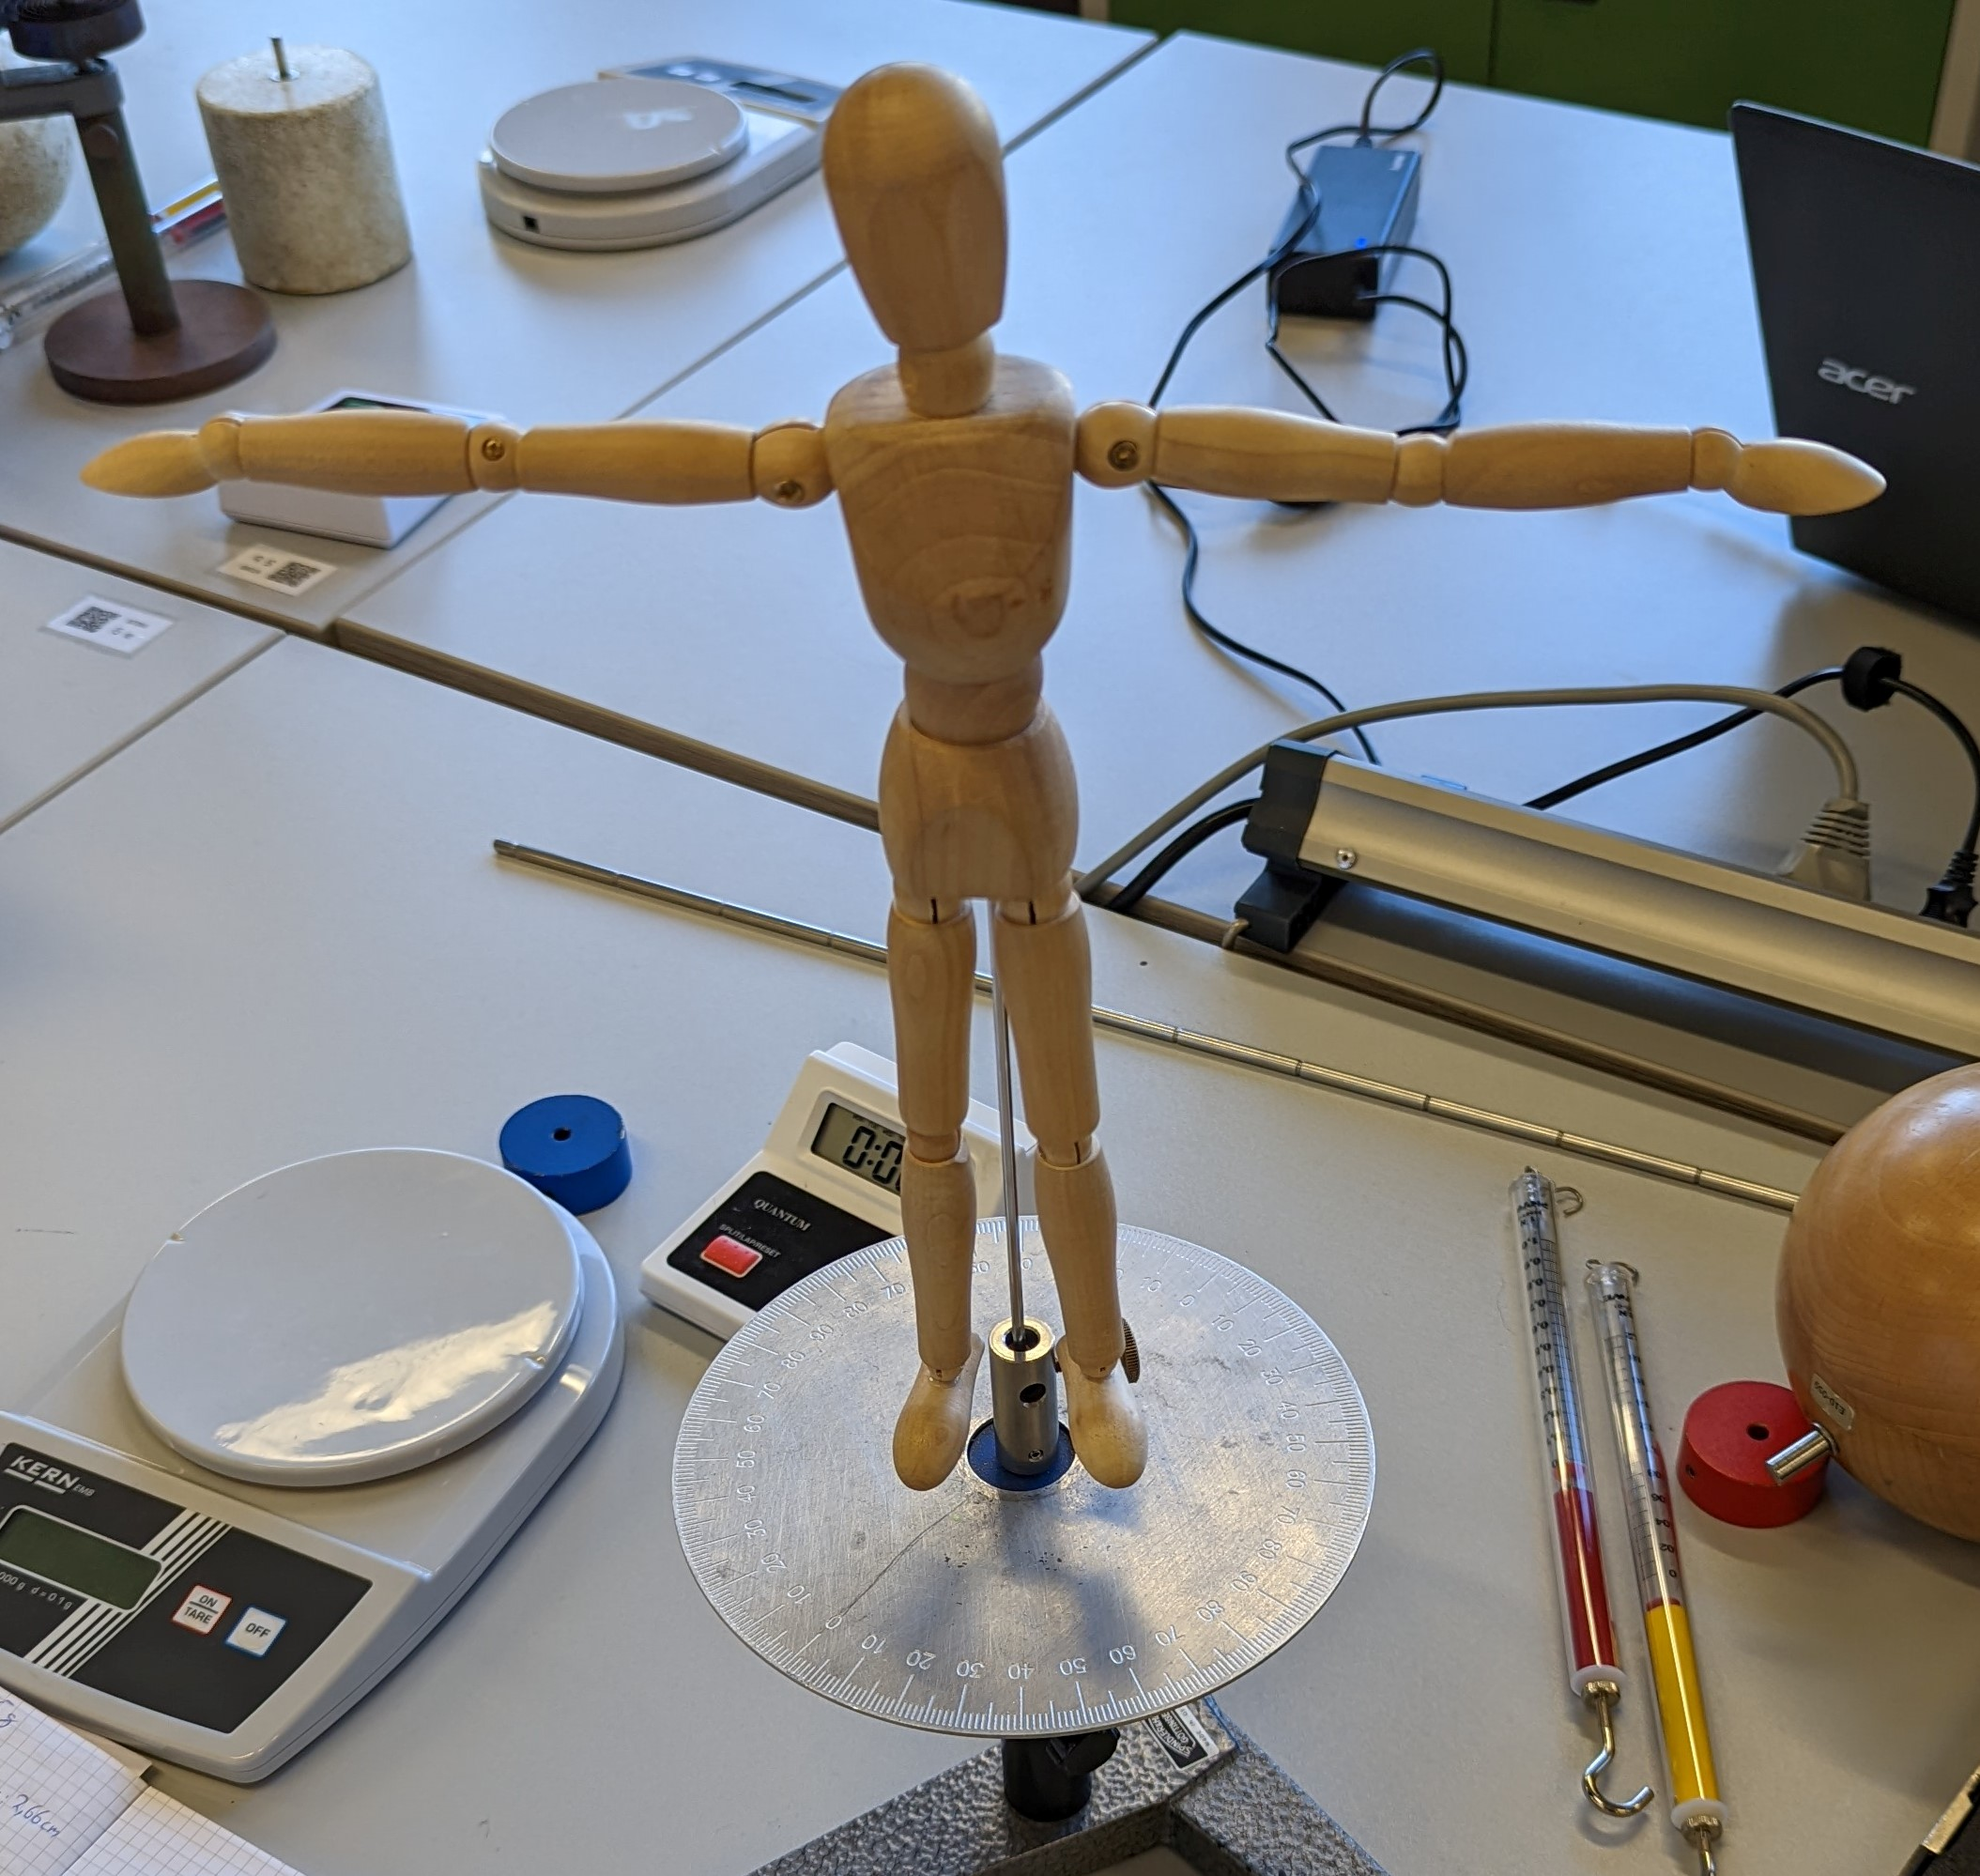
\includegraphics[width=0.8\textwidth]{content/T_Pose3.jpg}
        \caption{Stellung 2}
        \label{fig:D_Holzpuppe2}
    \end{subfigure}    
    \caption{Verschiedene Stellungen der Holzpuppe, welche auf der Drillachse montiert ist.}
    \label{fig:D_subfig}
\end{figure}